
\documentclass{acm_proc_article-sp}
%documentclass{article}
\begin{document}

\title{Paragraph: A Paravirtual Graphics Card in Palacios}
\numberofauthors{3} %  in this sample file, there are a *total*
\author{
% 1st. author
\alignauthor
Ruba Merza\\
       \affaddr{Northwestern University}\\
       \affaddr{1117 Forest Avenue}\\
       \affaddr{Evanston, IL, 60202}\\
       \email{ruba@u.northwestern.edu}
% 2nd. author
\alignauthor
Ross Freiman\\
       \affaddr{Northwestern University}\\
       \affaddr{2234 Sherman Ave.}\\
       \affaddr{Evanston, IL, 60201}\\
       \email{rossfreiman2013@u.northwestern.edu}
% 3rd. author
\alignauthor
Ketaki Joshi\\
       \affaddr{Northwestern University}\\
       \affaddr{1021 Dempster Street}\\
       \affaddr{Evanston ,IL 60201}\\
       \email{ketakijoshi2013@u.northwestern.edu}
}

\maketitle
\begin{abstract}
The focus of this paper is implementing a paravirtual graphics card and an X11 device driver for
a virtual machine monitor called Palacios. While Palacios implements a VGA graphics card with
a complex interface to the virtual guest, a paravirtual graphics card provides a simple interface
by writing directly an array of pixels into a chunk of memory, called the framebuffer, which is then
read by an X11 server and rendered onto the screen through an X11 client.
This paper looks at the current implementation of graphics in Palacios and describes the new
implementation with a paravirtual graphics card. It also provides a short description of the X
client\--­server model and the X11 driver written for the paravirtual graphics card.
\end{abstract}

\category{H.4}{Virtualization}{Systems}
\terms{Documentation, Design, Experimentation, Theory}
\keywords{Paravirtual, Graphics, Graphics Card, X11, Palacios, Virtual Device}

\section{Introduction}
The goal of this paper is to describe an implementation of a paravirtual
graphics card for Palacios, an OS independent open source virtual machine
monitor. \cite{techreport} Palacios is designed to be 
highly configurable and provides a suitable environment
for prototyping new extensions and devices. \cite{techreport} Palacios currently implements
  a virtual VGA card whose interface to the guest VM is very elaborate. The
  purpose of a paravirtual graphics card is to eliminate such complex interface
  by providing a much simpler and more compact one to the guest that can
  consequently make for a substitute for the VGA card altogether. In addition to
  replacing the VGA in Palacios, the paravirtual graphics card's manageable
  interface makes it easy to configure it with an X11 device driver and thus
  enables us to harness the capabilities of the X11 window system and run it with the
  graphics card within a virtual guest. In the following sections we go into
  detail about Palacios' current implementation of graphics, the paravirtual
  graphics card's interface, the X11 window system, and the steps we took in
  building such graphics card and running X on a virtual guest.

\section{Graphics in Palacios}
The way graphics currently work on Palacios comprises of three main components.
The VGA device, the graphics console, and the VNC server/client. In the
following subsection we will give an overview of the VGA device, followed by two
subsections, one describing the graphics console and the other describing the
VNC server/client used in Palacios.

\begin{figure}[h]                                              
\centering                                                 
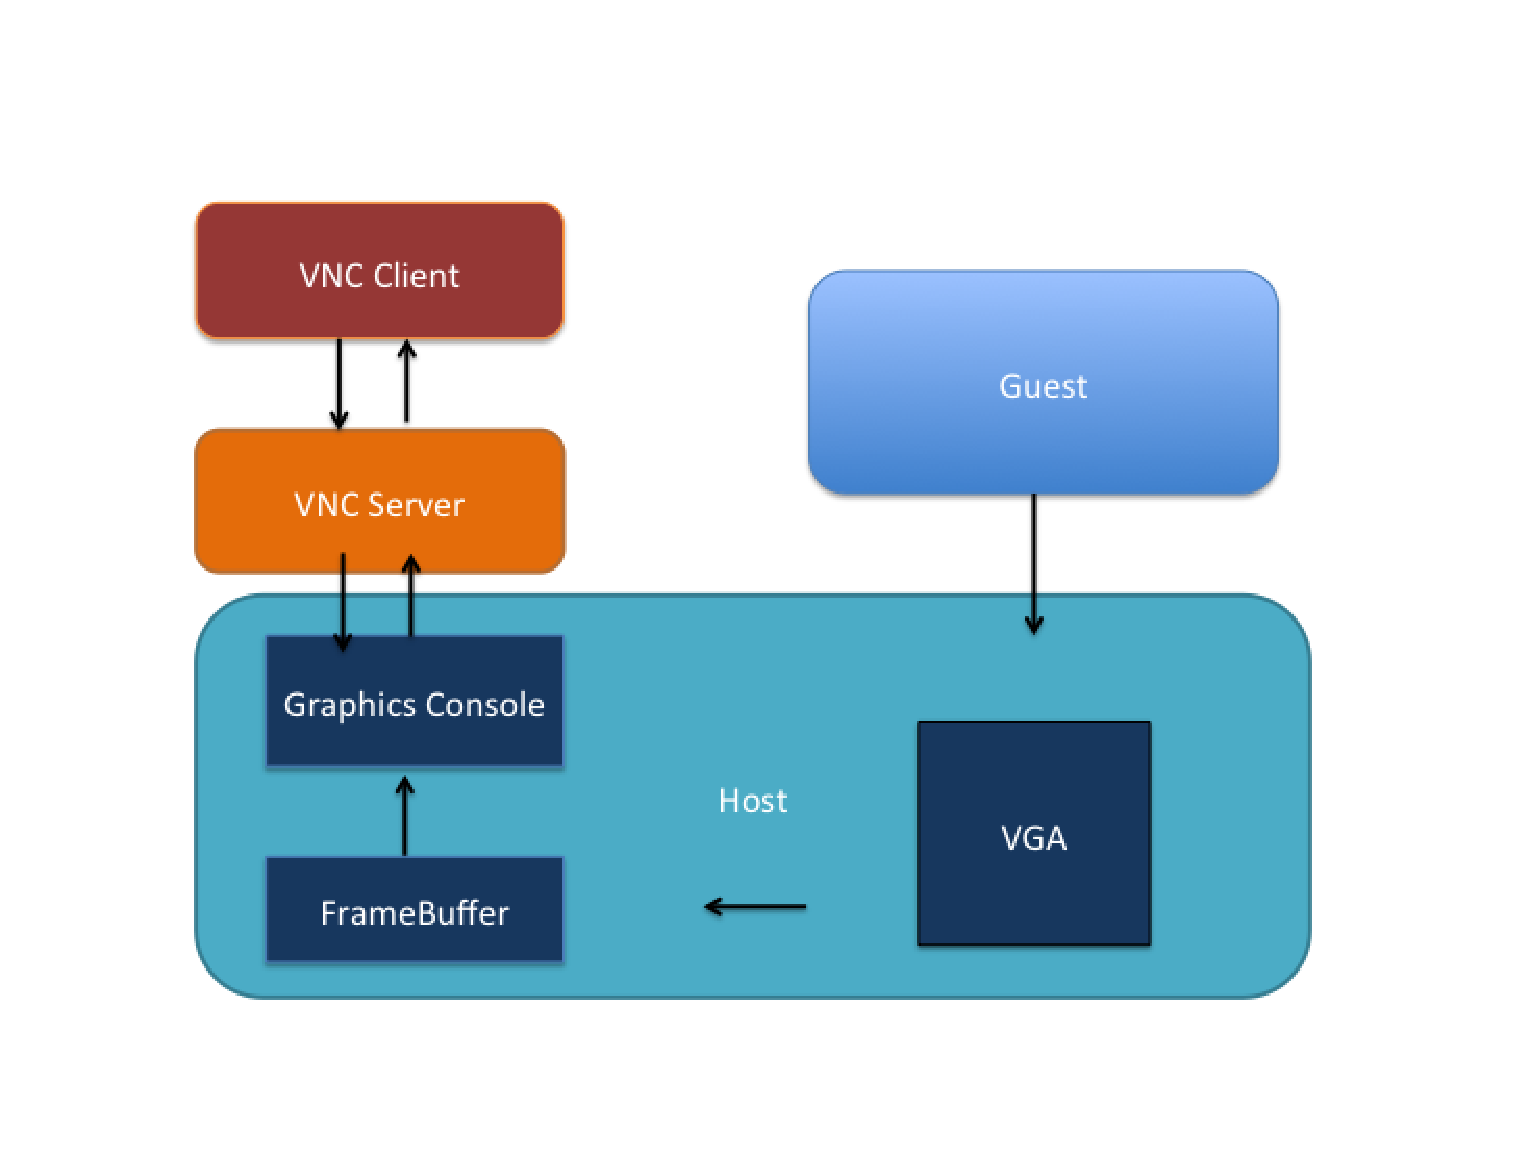
\epsfig{file=VGA.eps, height=3in, width=4in}                                      
\caption{A model of how graphics work currently in Palacios}   
\end{figure}                                               

\subsection{VGA}
\subsubsection{What is VGA?}
Palacios currently uses an emulated Video Graphics Array (VGA) device for graphics. VGA is a display standard that was first developed by IBM in 1987 for their PS/2 computers. It was used as an interface between a computer monitor and the hardware. It gave users the ability to operate in one of two display modes at a time; either a 640x480  resolution display with up to 16 colors or a lower resolution display of 320x200 but with up to 256 colors available. Today, the successors of VGA are still in wide-use by graphic cards, but they are slowly becoming replaced as DVI (Digital Visual Interfaces) and HDMI (High-Definition Multimedia Interface) become more popular.
\par
To connect to a monitor, the hardware used a 15-pin connector that allowed communication through signals between the monitor and the VGA device. As seen in Figure 2, each color (red, green, blue) has a dedicated pin for data to flow through as well as specific pins for vertical sync and horizontal sync. Vertical and horizontal sync are digital signals whereas the colors are analog, and used for synchronization of the display. The vertical sync tells a monitor to display a new image and the horizontal sync tells the monitor to refresh a single row of pixels. In the case of VGA 640x480 resolution, each row would be of size 640 pixels and 480 horizontal syncs would be sent before the entire screen is drawn. Once a vertical sync pulse is received, the monitor starts to draw back at its upper-left hand corner. These synchronization pulses sent by the video card are extremely important for creating and maintaining stable images on the screen. Pins 5 through 10, excluding pin 9, are used as grounds for the colors and syncs. The other pins (4, 11, 12, \& 15) are called “monitor ID” pins that send information to the video card about what type of monitor it is connected to. Pin 9 is actually plugged and not used for anything, except in helping align the other pins with their respective sockets. 
\par
 In terms of how it works, VGA maintains an internal buffer where it holds the contents of the screen. This internal buffer maintains an array of pixels, representing the screen and this array is written into every time the screen needs to be updated. Thus this buffer always has an updated version of the screen contents.
 \par
 Figure 3 is an interesting analog to Palacios, but is not completely accurate as to what Palacios and the VGA are doing. The guest believes its writing into the frame buffer through the VGA device and thus writing the content onto the screen. In the case of the VGA, the number of bits for each color will be 1, if it is in 16 color mode, since only 4 bits are needed for 16 different combinations. The last bit is most likely used for opacity, i.e. how transparent the pixel is. In VGA, for 256 color mode, there are 8 bits used. However, instead of each bit corresponding to some color, the bits were an index into a map of colors that allowed for use 6 different bits to be used for each color. While only 256 colors could be shown at any one time, a much larger palette of colors is available to choose the colors from. In actuality, each color could use 8-bits thus effectively having a palette of 2\textsuperscript{24} different colors, but the original VGA chose only to have 6-bits per color in the map. Instead of actually having the VGA have a frame buffer to write into, its memory that is written on is then copied into the frame buffer in Palacios graphics console which serves as the interface between the VNC server and Palacios in getting pixels to be written onto the screen. 
 
 \subsubsection{Why try to replace VGA?}
 VGA was very impressive for the time in which it was developed and was the predecessor to want display standards still used today. However, VGA presents a very complex interface due to the fact that it was created in a time when memory was scarce and processing power was much smaller. The intricacy of the device allowed it run when resources were limited. However, the basic principle of the interface was to have an array of pixels to be written into and then the data about the pixels would be sent to the screen and be displayed. Unfortunately, Palacios has to deal with the convolution that this legacy interface imposes. In addition, trying to use more current interfaces may seem like a way to lower the barrier of complexity since they usually have plenty of resources to be utilized. However, hardware now has advanced such that displays are more complicated due to trying to make processes even faster and more powerful than they already are. As such a simple interface such as just an area of memory to write in provides an effective way for graphics in Palacios to work.  
 
\begin{figure}                                              
\centering                                                     
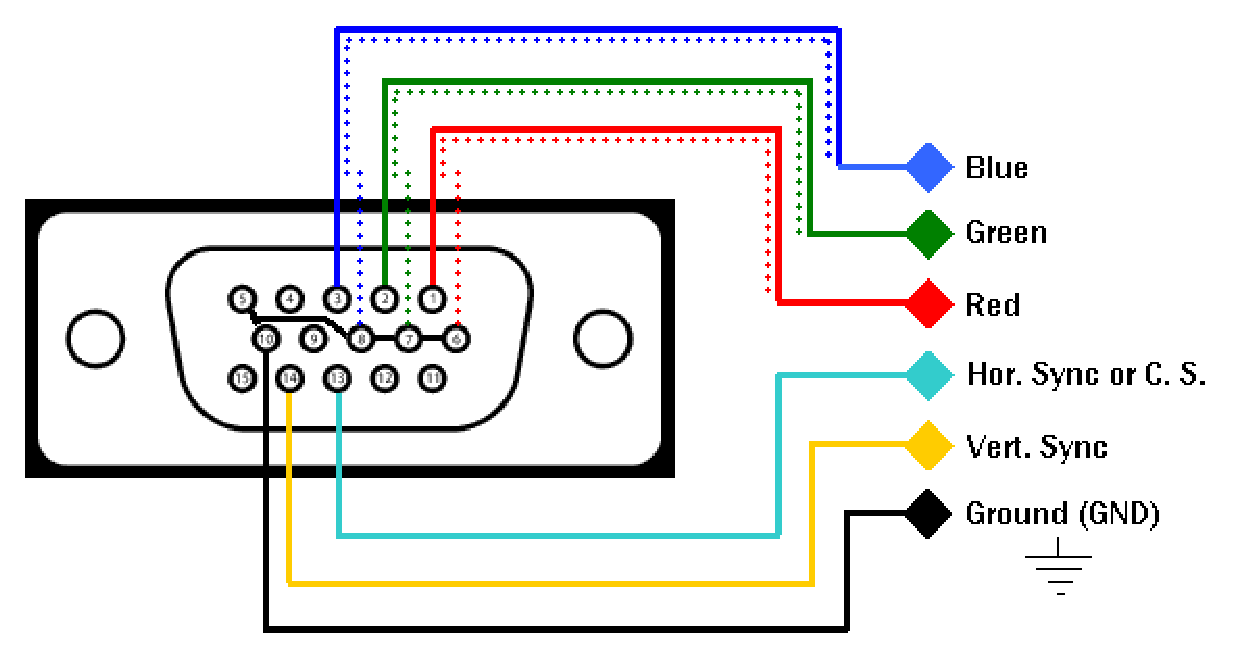
\epsfig{file=vga-head.eps, height=6cm, width=9cm}                   
\caption{VGA Connector Socket}   
\end{figure} 

\begin{figure}                                              
\centering                                                     
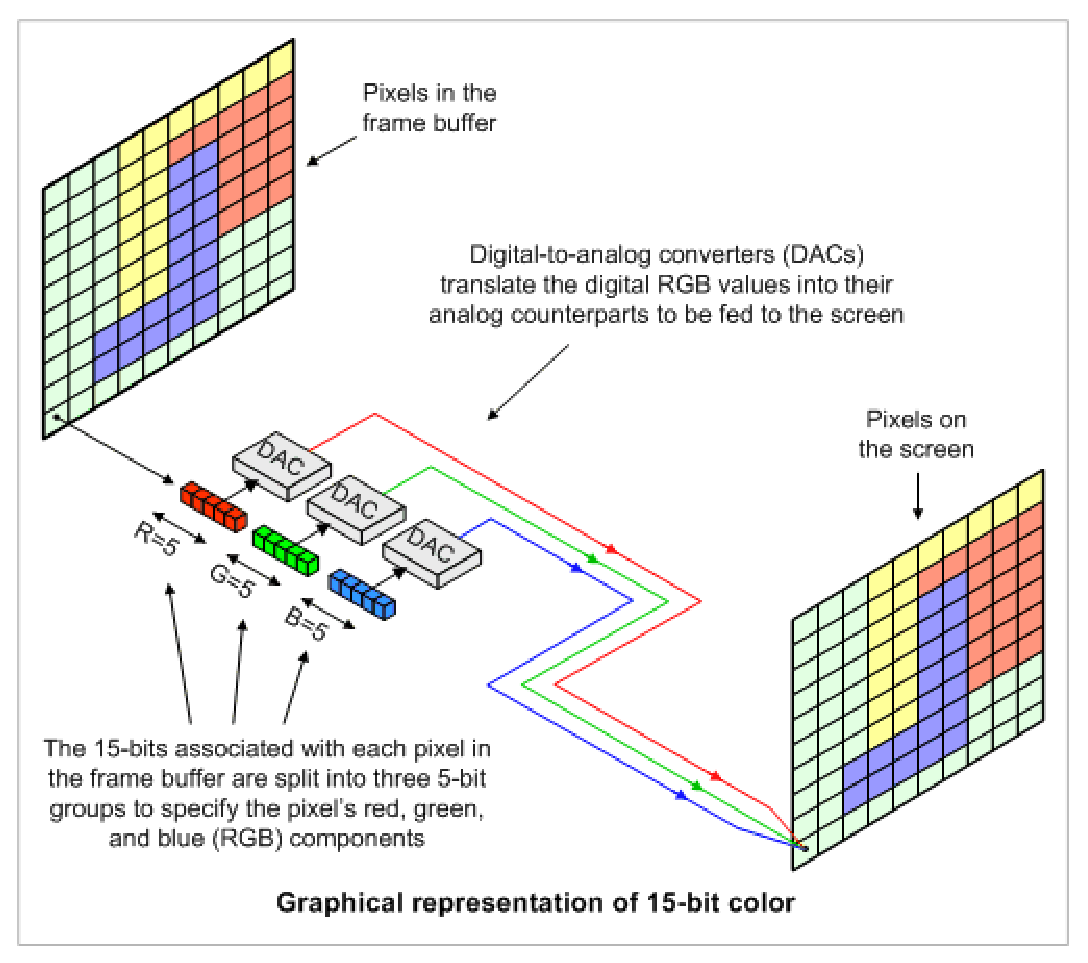
\epsfig{file=framebuf_toscreen.eps, height=9cm, width=9cm}                   
\caption{Flow of Pixel Data from Frame Buffer to Screen}   
\end{figure} 

\subsection{The Graphics Console} % can add more about its functions
The Graphics Console interface interfaces with a VM's text\--mode and graphics
mode display adaptor (e.g. VGA), keyboard, and mouse to allow the host OS to display the VM
console as appropriate. In the Linux module, the graphics console interface implementation provides
for a userspace utility to attach to a frame buffer. The utility then exports this frame buffer, keyboard,
and mouse to remote clients through the VNC protocol. \cite{techreport}

\subsection{VNC}
Palacios uses a Virtual Network Computing (VNC) server and a VNC client to
display the guest's screen. The VNC client makes a request to the VNC server to view the screen. 
The VNC server uses a special system call to request an array of pixels representing the whole screen from Palacios. 
Palacios copies into that array (frame buffer) from an internal array that it
maintains. By connecting to the VNC server, Palacios's graphics console exports
the frame buffer to a VNC client which connects to the VM at a certain port and
displays the screen with the contents of that frame buffer.

\section{Our method}
After describing the interaction between Palacios's VGA virtual device, graphics console and the VNC server and client, we now go into detail
about the paravirtual graphics card (Paragraph) that we built to replace the VGA 
device. We also discuss the addition of an X11 server and X11 device driver to
the virtual guest. Figure 2 shows the new addition of Paragraph and X11 to
Palacios and the interaction between these new components on the guest and host
machines. 
\par
When an X11 client is run on the guest (such as xterm for example), it talks to
an X11 server. The X server needs the address of a frame buffer onto which it
draws pixel values. It gets the address of that frame buffer through the device
driver it is configured to use (in our case, the Paragraph device driver). The 
driver searches for the device, and enables it to be written on by the X11
server.  Once Paragraph has data written to it, it renders a
screen display to the graphics console in Palacios, which stores it in memory
and allows host user access to it. The VNC server uses this access to make the 
screen contents available via the VNC protocol. The VNC client connects to the 
VNC server, gets the content and displays on screen.
\begin{figure}[h]                                              
\centering                                                     
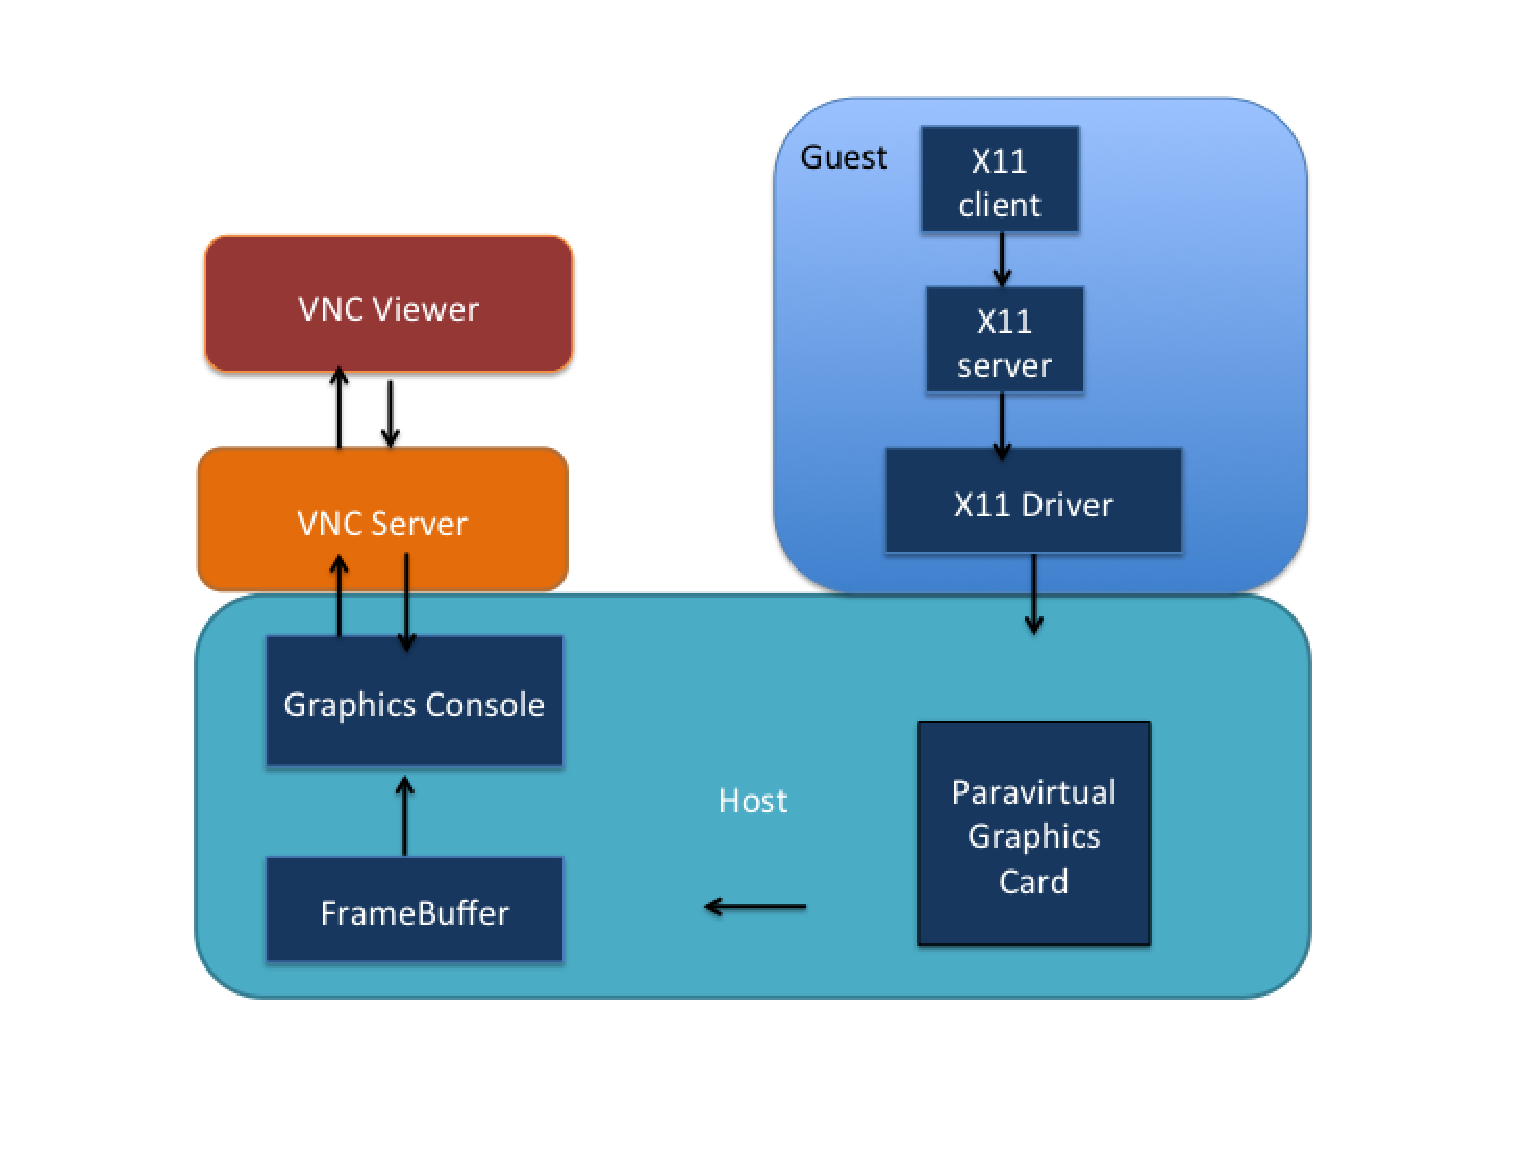
\epsfig{file=Paragraph.eps, height=3in, width=4in}                   
\caption{The new model of graphics in Palacios}   
\end{figure}                                                   
\subsection{ParaGraph: The Paravirtual Graphics Card}
A paravirtual graphics card is essentially a way of representing a graphics card
interface to a virtual guest that is similar but not identical to its hardware
implementation. In our case, we have Paragraph, a virtual graphics card device
that offers the guest a very straightforward interface which is simply: write
the array of pixels. Paragraph's configuration specifies how to write to the
internal array of pixels that Palacios uses to copy from into the frame buffer
that is maintained by the graphics console. \\
\subsubsection{Data Structures}
In order to register Paragraph as a PCI device on the guest, a struct was used
to represent and store Paragraph's state. The struct stores information such as
Paragraph's physical address in the guest, and the size of its mapped region in
pages. It also maintains records regarding the VM, the PCI bus, the VM devices and PCI
devices. If Paragraph is configured to be used as memory, fields for its
physical and virtual addresses are used to store such information. If the
graphics console is used for memory, then the appropriate spec information is
also kept in the paragraph state struct. 
\subsubsection{Configuration}
Paragraph can be set to 1 of 3 modes: \\
\begin{enumerate}
\item MEM: Paragraph is used directly as backing memory on which the pixel values
are stored.
\item GCONS\textunderscore MEM: Paragraph is used as backing memory but its contents are
then rendered to the graphic console's frame buffer.
\item GCONSD\textunderscore DIRECT: The graphics console is used directly as memory.
\end{enumerate}
When Paragraph is configured to MEM mode, it can be mapped into a chunk of
memory (mmap) and then written to directly. Whatever is written to it will be
passed on to the VNC server and displayed on the screen. When Paragraph is set
to GCONS\textunderscore MEM, whatever gets written on Paragraph will then be
copied to the graphic console's frame buffer (memcpy) and the VNC server will
display its contents on Screen. Finally, if Paragraph is set to GCONS
\textunderscore DIRECT, nothing will be written on the device, the graphic
console will be written to directly.

The Paragraph device projects a graphics console to the guest as a PCI device
Paragraph's length was configured to 4MB and it was given the physical address
of 0x80000000. Paragraph's implementation includes the required initialization
such as registering it as a PCI device and initializing the PCI BAR. 
%%%% table with paragraph functions?
Paragraph's implementation is less than 300 lines of code.

\subsection{X11}
 X11 is a computer software system and network protocol that provides a basis for graphical user interfaces (GUIs) and rich input device capability for networked computers.X11 uses a client-server protocol, the X protocol. The server is the computer or X terminal with the screen, keyboard, mouse and server program and the clients are application programs. Clients may run on the same computer as the server or on a different computer, communicating over Ethernet via TCP/IP protocols.An X server communicates with various client programs. The server accepts requests for graphical output (windows) and sends back user input (from keyboard, mouse, or touchscreen).
 A major feature of X is network transparency, which means that any X client can run either on the local machine or on a remote machine without any obvious difference to the user in most cases.  
 Figure 5 shows the client-server interaction in X11.
 \begin{figure}[h]
 \centering
 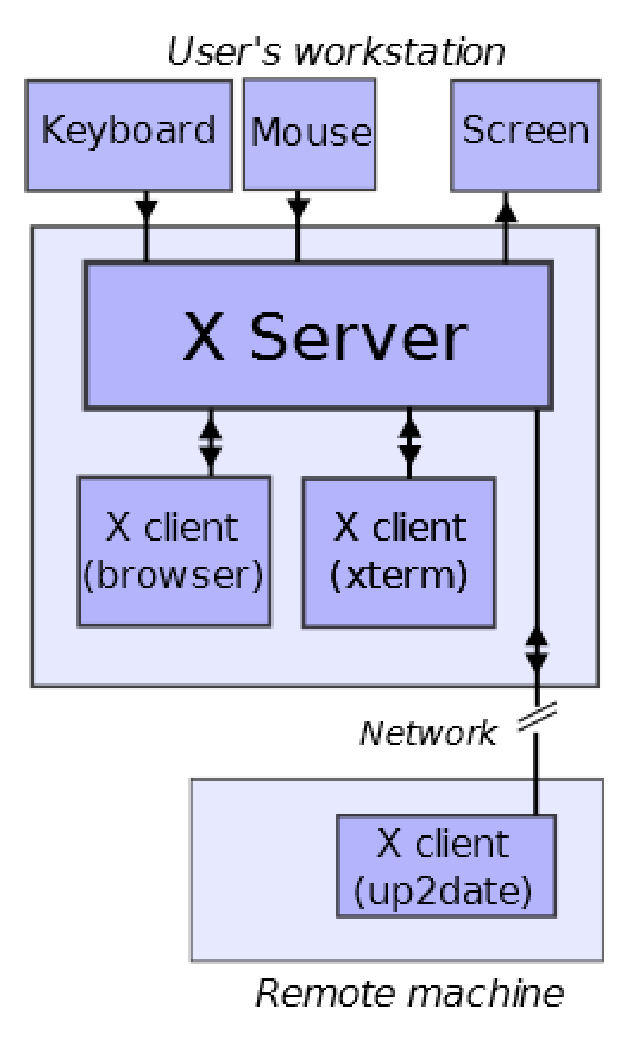
\epsfig{file=X11.eps, height=3in, width=2in}
 \caption{X11 Client-Server model}
 \end{figure}
\subsubsection{X11 device driver for Paragraph}
The X11 server requires device drivers to identify and communicate with devices.
In our case, we needed to write a device driver for Paragraph which the X server can
write onto.
X11 drivers come with a set of mandatory functions that they must perform. Table
1 lists these functions. 
Due to Paragraph's straightforward and simple interface, the device driver only
needed slight editing in order for it to communicate with paragraph. A simple
mmap function was used to map paragraph to a chunk of memory and return
paragraph's virtual address, which would consequently be used as the frame
buffer's base address. The X11 server writes to the memory at that address. 
\section{Results}
The goal of this project was to write a paravirtual graphics card and run an X11
client on the guest that uses this graphics card. Professor Dinda aided us
greatly by providing us with a Paragraph framework that helped us in the first
part, as for running an X11 client, we ran into many issues due to our lack of
experience with X. XWe were able to create a paravirtual graphics card device
that can be configured. 
We were also able to configure an X11 device driver that used such a device as a
frame buffer for the X11 server to render to. However, we still have not been able to run
the X server on the guest, mainly due to our use of a fairly limited guest OS
that don't have all the devices or libraries that the X server needs.
\section{Outstanding Issues}
Running the X server on the virtual guest requires it to be reconfigured. The
use of another guest that has pseudo terminals installed. A
\textit{pseudo\textunderscore terminal} is a special interprocess communication
channel that acts like a terminal. One end of the channel is called the master side or master pseudo-terminal device, 
the other side is called the slave side. 
Data written to the master side is received by the slave side as if it was the result of a user typing at an ordinary terminal, 
and data written to the slave side is sent to the master side as if it was written on an ordinary terminal.
X11 clients such as xterm use pseudo terminals to implement their terminal emulation functionality.


\begin{table}
 \centering
  \caption{X11 Driver Functions}
  \begin{tabular}{|l|p{4cm}|} \hline
  \textbf{Function Name}&\textbf{Description}\\ \hline
  ScreenInit & An initialisation function is called from the DIX layer for each screen at the start of each server generation.\\ \hline
  Probe & Identify if there is any hardware present that the driver knows how to drive.\\ \hline
  PreInit & Process information from the xorg.conf file, determine the full characteristics of the hardware, and determine if a valid configuration is present. \\ \hline
  Mode Switch & Change video mode \\ \hline
  ViewPort change & Change the origin of the physical view port \\ \hline
  ScreenSaver state change & Screen saver activation/deactivation \\ \hline
  CloseScreen & A close screen function is called from the DIX layer for each screen at the end of each server generation \\ \hline
\end{tabular}
\end{table}


\section{Acknowledgments}
We would like to thank Peter Dinda for the many, many hours he spent tirelessly with us as we
tried to get the X server running on the virtual guest, and for all the
resources and frameworks he provided us with. We would also like to thank Kyle
Hale for sending us all the different guest OS's and reconfiguring them for us
whenever we needed them. Thanks to our diligent undergraduate assistants Prem
Seetharaman, Jack Hudson, and Josiah Matlack for putting up with us during and
not during their office hours.
%
% The following two commands are all you need in the
% initial runs of your .tex file to
% produce the bibliography for the citations in your paper.
%\bibliographystyle{abbrv}
%\bibliography{sigproc}  % sigproc.bib is the name of the Bibliography in this case
% You must have a proper ".bib" file
%  and remember to run:
% latex bibtex latex latex
% to resolve all references
%
% ACM needs 'a single self-contained file'!
%\balancecolumns
\begin{thebibliography}{1}

  \bibitem{techreport} Lange, Jack, Peter Dinda, Kyle Hale, and Lei Xia. An Introduction to the Palacios Virtual Machine Monitor---Version 1.3. Tech. Northwestern University, 11 Nov. 2011. Web. 01 Mar. 2013.

  \bibitem{impj}  The 

  \bibitem{norman} E. H. Norman {\em Japan's emergence as a modern
  state} 1940: International Secretariat, Institute of Pacific
  Relations.

  \bibitem{fo} Bob Tadashi Wakabayashi {\em Anti-Foreignism and Western
  Learning in Early-Modern Japan} 1986: Harvard University Press.

  \end{thebibliography}
Generated by bibtex from your ~.bib file.  Run latex,
then bibtex, then latex twice (to resolve references)
the command \texttt{{\char'134}thebibliography}.
% This next section command marks the start of
% Appendix B, and does not continue the present hierarchy
\balancecolumns
% That's all folks!
\end{document}
